\chapter{Universal Serial Bus}

This chapter presents an overview of the \acrfull{USB} Full Speed interface, with focus on the features used in the GEX firmware. \gls{USB} is a versatile and powerful interface which replaces several older technologies; for this reason its specification is very complex and going into all details is hardly possible. We will cover the basic principles and terminology of \gls{USB} and focus on the parts relevant for the GEX project. More information about the bus can be found in the official specification~\cite{usbif-spec}, related documents published by the USB Implementers Forum, and other on-line resources~\cite{usb-nutshell,usb-made-simple}.

\section{Basic Principles and Terminology}

\begin{figure}[h]
	\centering
	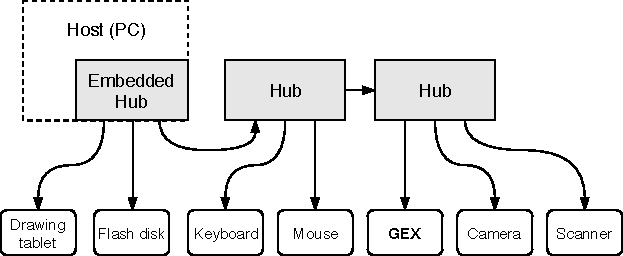
\includegraphics[scale=1] {img/usb-hierarchy-redraw.pdf}
	\caption[USB hierarchical structure]{\label{fig:usb-hierarchy}The hierarchical structure of the USB bus}
\end{figure}

\gls{USB} is a hierarchical bus with a single master (\textit{host}) and multiple slave devices. A \gls{USB} device that provides functionality to the host is called a \textit{function}~\cite{usb-function}.

\subsection{Pipes and Endpoints}

Communication between the host and a function is organized into virtual channels called \textit{pipes} connecting to the device's \textit{endpoints}, identified by endpoint numbers.

\begin{figure}[h]
	\centering
	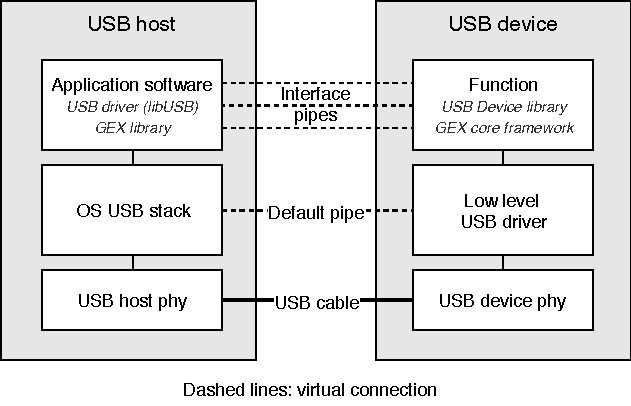
\includegraphics[scale=1] {img/usb-logical-redraw.pdf}
	\caption{\label{fig:usb-logical}The logical structure of USB}
\end{figure}

Endpoints can be either unidirectional or bidirectional; the direction from the host to a function is called OUT, the other direction (function the host) is called IN. A bidirectional endpoint is technically composed of a IN and OUT endpoint with the same number. All transactions (both IN and OUT) are initiated by the host; functions have to wait for their turn. Endpoint 0 is bidirectional, always enabled, and serves as a \textit{control endpoint}. The host uses the control endpoint to read information about the device and configure it as needed.

\subsection{Transfer Types}

There are four types of data transfers defined in \gls{USB}: control, bulk, isochronous, and interrupt. Each endpoint is configured for a fixed transfer type:

\begin{itemize}
	\item \textit{Control} -- initial configuration after device plug-in; also used for other aplication-specific control messages that can affect other pipes.
	\item \textit{Bulk} -- used for burst transfers of large messages
	\item \textit{Isochronous} -- streaming with guaranteed low latency; designed for audio or video streams where some data loss is preferred over stuttering
	\item \textit{Interrupt} -- low latency short messages, used for human interface devices like mice and keyboards
\end{itemize}

\subsection{Interfaces and Classes}

The function's endpoints are grouped into \textit{interfaces}. An interface describes a logical connection of endpoints, such as the reception and transmission endpoints that belong together. An interface is assigned a \textit{class} defining how it should be used.

Standard classes are defined by the USB specification~\cite{usb-class-list} to provide a uniform way of interfacing devices of the same type, such as human-interface devices (mice, keyboards, gamepads) or mass storage devices. The use of standard classes makes it possible to re-use the same driver software for devices from different manufacturers.

The class used for the GEX's ``virtual COM port'' function was originally meant for telephone modems, a common way of connecting to the Internet at the time the first versions of USB were developed. A device using this class will show as \verb|/dev/ttyACM0| on Linux and as a COM port on Windows, provided the system supports it natively or the right driver is installed.

\subsection{Descriptors}

USB devices are introspectable, that is, the host can learn about a newly connected device automatically by probing it, without any user interaction. This is accomplished using a \textit{descriptor table}, a binary structure stored in the function and read by the host through the control endpoint (default pipe) after the device is attached.

Each descriptor starts with a declaration of its length (in bytes), followed by its type,  allowing the host to skip unknown descriptors without having to discard the rest of the table. The descriptors are logically nested and form a tree-like structure, but they are stored sequentially in the descriptor table and the lengths do no include sub-descriptors.

The topmost descriptor holds information about the entire function, including the vendor and product IDs which uniquely identifies the device model. It is followed by a Configuration descriptor, grouping a set of interfaces. More than one configuration may be present and available for the host to choose from; however, this is rarely used or needed. Each configuration descriptor is followed by one or more interface descriptors, each with its class-specific sub-descriptors and/or endpoint descriptors.

The descriptor table used by GEX is captured in \cref{fig:gex-descriptors} for illustration. The vendor and product IDs were obtained from the pid.codes repository~\cite{pidcodes} providing free product codes to open source projects. The official way of obtaining the unique code involves high recurring fees (\$4000 per annum) to the USB Implementers Forum, Inc. and is therefore not affordable for non-commercial use; alternatively, a product code may be obtained from some \gls{MCU} vendors if their product is used in the device.
\newpage

\hspace*{-1.5em}
\begin{minipage}[t]{0.5\textwidth}\scriptsize
\begin{verbatim}
Device Descriptor:
  bLength                18
  bDescriptorType         1
  bcdUSB               2.00
  bDeviceClass          239 Miscellaneous Device
  bDeviceSubClass         2 
  bDeviceProtocol         1 Interface Association
  bMaxPacketSize0        64
  idVendor           0x0483 STMicroelectronics
  idProduct          0x572a 
  bcdDevice            0.01
  iManufacturer           1 MightyPork
  iProduct                2 GEX
  iSerial                 3 0029002F-42365711-32353530
  bNumConfigurations      1
  Configuration Descriptor:
    bLength                 9
    bDescriptorType         2
    wTotalLength           98
    bNumInterfaces          3
    bConfigurationValue     1
    iConfiguration          0 
    bmAttributes         0x80
      (Bus Powered)
    MaxPower              500mA
    Interface Descriptor:
      bLength                 9
      bDescriptorType         4
      bInterfaceNumber        0
      bAlternateSetting       0
      bNumEndpoints           2
      bInterfaceClass         8 Mass Storage
      bInterfaceSubClass      6 SCSI
      bInterfaceProtocol     80 Bulk-Only
      iInterface              4 Settings VFS
      Endpoint Descriptor:
        bLength                 7
        bDescriptorType         5
        bEndpointAddress     0x81  EP 1 IN
        bmAttributes            2
          Transfer Type            Bulk
          Synch Type               None
          Usage Type               Data
        wMaxPacketSize     0x0040  1x 64 bytes
        bInterval               0
      Endpoint Descriptor:
        bLength                 7
        bDescriptorType         5
        bEndpointAddress     0x01  EP 1 OUT
        bmAttributes            2
          Transfer Type            Bulk
          Synch Type               None
          Usage Type               Data
        wMaxPacketSize     0x0040  1x 64 bytes
        bInterval               0
    Interface Association:
      bLength                 8
      bDescriptorType        11
      bFirstInterface         1
      bInterfaceCount         2
      bFunctionClass          2 Communications
      bFunctionSubClass       2 Abstract (modem)
      bFunctionProtocol       1 AT-commands (v.25ter)
      iFunction               5 Virtual Comport ACM
\end{verbatim}
\end{minipage}\hspace{1em}
\begin{minipage}[t]{0.5\textwidth}\scriptsize
\begin{verbatim}
    Interface Descriptor:
      bLength                 9
      bDescriptorType         4
      bInterfaceNumber        1
      bAlternateSetting       0
      bNumEndpoints           1
      bInterfaceClass         2 Communications
      bInterfaceSubClass      2 Abstract (modem)
      bInterfaceProtocol      1 AT-commands (v.25ter)
      iInterface              5 Virtual Comport ACM
      CDC Header:
        bcdCDC               1.10
      CDC Call Management:
        bmCapabilities       0x00
        bDataInterface          2
      CDC ACM:
        bmCapabilities       0x06
          sends break
          line coding and serial state
      CDC Union:
        bMasterInterface        1
        bSlaveInterface         2 
      Endpoint Descriptor:
        bLength                 7
        bDescriptorType         5
        bEndpointAddress     0x83  EP 3 IN
        bmAttributes            3
          Transfer Type            Interrupt
          Synch Type               None
          Usage Type               Data
        wMaxPacketSize     0x0008  1x 8 bytes
        bInterval             255
    Interface Descriptor:
      bLength                 9
      bDescriptorType         4
      bInterfaceNumber        2
      bAlternateSetting       0
      bNumEndpoints           2
      bInterfaceClass        10 CDC Data
      bInterfaceSubClass      0 
      bInterfaceProtocol      0 
      iInterface              6 Virtual Comport CDC
      Endpoint Descriptor:
        bLength                 7
        bDescriptorType         5
        bEndpointAddress     0x02  EP 2 OUT
        bmAttributes            2
          Transfer Type            Bulk
          Synch Type               None
          Usage Type               Data
        wMaxPacketSize     0x0040  1x 64 bytes
        bInterval               0
      Endpoint Descriptor:
        bLength                 7
        bDescriptorType         5
        bEndpointAddress     0x82  EP 2 IN
        bmAttributes            2
          Transfer Type            Bulk
          Synch Type               None
          Usage Type               Data
        wMaxPacketSize     0x0040  1x 64 bytes
        bInterval               0
\end{verbatim}
\end{minipage}\vspace{-1em}
\begin{figure}[H]
	\cprotect\caption{USB descriptors of a GEX prototype obtained using \verb|lsusb -vd vid:pid|}
\end{figure}


\section{USB Physical Layer}

\gls{USB} uses differential signaling with \gls{NRZI} encoding and bit stuffing (the insertion of dummy bits to prevent long intervals in the same \gls{DC} level). The encoding, together with frame formatting, checksum verification, retransmission, and other low-level aspects of the \gls{USB} connection are entirely handled by the \gls{USB} physical interface block in the microcontroller's silicon. Normally we do not need to worry about those details; nonetheless, a curious reader may find more information in chapters 7 and 8 of~\cite{usbif-spec}. What needs our attention are the electrical characteristics of the physical connection, which need to be understood correctly for a successful schematic and \gls{PCB} design.

The \gls{USB} cable contains 4 conductors: V$_\mathrm{BUS}$ (+5\,V), D+, D--, and \gls{GND}. The data lines, D+ and D--, are also commonly labeled DP and DM. This differential pair should be routed in parallel on the \gls{PCB} and kept at the same length.

\gls{USB} versions that share the same connector are backward compatible. The desired bus speed is requested by the device using a 1.5\,k$\Omega$ pull-up resistor to 3.3\,V on one of the data lines: D+ pulled high for Full Speed (shown in \cref{fig:usb-pullup-fs}), D-- pulled high for Low Speed. The polarity of the differential signals is also inverted depending on the used speed, as the idle level changes. Some microcontrollers integrate the correct pull-up resistor inside the \gls{USB} peripheral block (including out STM32F072), removing the need for an external resistor.

\begin{figure}[h]
	\centering
	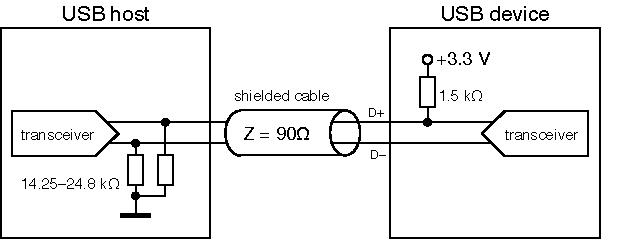
\includegraphics[scale=1]{img/usb-resistors.pdf}
	\caption[USB pull-ups]{\label{fig:usb-pullup-fs}Pull-up and pull-down resistors near the host and a Full Speed function, as prescribed by the USB specification rev. 2.0}
\end{figure}

When a function needs to be re-enumerated by the host, which causes a reload of the descriptor table and the re-attachment of software drivers, it can momentarily remove the pull-up resistor, which the host will interpret as if the device was disconnected. With an internal pull-up, this can be done by flipping a bit in a control register. An external resistor may be connected through a transistor controlled by a \gls{GPIO} pin. As discussed in~\cite{eev-gpio-pu}, a GPIO pin might be used to drive the pull-up directly, though this has not been verified by the author.

The V$_\mathrm{BUS}$ line supplies power to \textit{bus-powered} devices. \textit{Self-powered} devices can leave this pin unconnected and instead use an external power supply. The maximal current drawn from the V$_\mathrm{BUS}$ line is configured using a descriptor and should not be exceeded, but experiments suggest this is often not enforced.

\noindent More details about the electrical and physical connection may be found in~\cite{usb-nutshell}, sections \textit{Connectors} through \textit{Power}.

\section{USB Classes}

This section explains the classes used in the GEX firmware. A list of all standard classes with a more detailed explanation can be found in~\cite{usb-class-list}.

\subsection{Mass Storage Class} \label{sec:msc}

The \gls{MSC} is supported by all modern operating systems (MS Windows, MacOS, GNU/Linux, FreeBSD etc.) to support thumb drives, external disks, memory card readers and other storage devices.

%http://www.usb.org/developers/docs/devclass_docs/Mass_Storage_Specification_Overview_v1.4_2-19-2010.pdf
%http://www.usb.org/developers/docs/devclass_docs/usbmassbulk_10.pdf

The \gls{MSC} specification~\cite{usbif-msco} defines multiple \textit{transport protocols} that can be selected using the descriptors. The \gls{BOT}~\cite{usbif-bot} will be used for its simplicity. \gls{BOT} uses two bulk endpoints for reading and writing blocks of data and for the exchange of control commands and status messages.

For the mass storage device to be recognized by the host operating system, it must also implement a \textit{command set}. Most mass storage devices use the \textit{\gls{SCSI} Transparent command set}
\footnote{To confirm this assertion, the descriptors of five thumb drives and an external hard disk were analyzed using \verb|lsusb|. All but one device used the SCSI command set, one (the oldest thumb drive) used \textit{SFF-8070i}. A list of possible command sets can be found in~\cite{usbif-msco}}.

Unfortunately, the \gls{SCSI} Transparent command set appears to have been deliberately left unspecified for license or copyright reasons (see discussion in~\cite{usb-tscsi-wtf} and the surrounding thread) and the protocol now used under this name is an industry standard without a clear definition. Some pointers may be found in~\cite{usb-tscsi} and by examining the source code of the USB Device driver library provided by ST Microelectronics.

This command set lets the host read information about the attached storage, such as its capacity, and check for media presence and readiness to write or detach. This is used, e.g., for the ``Safely Remove'' function, which ensures that all internal buffers have been written to Flash.

In order to emulate a mass storage device without having a physical storage medium, we need to generate and parse the file system on-the-fly as the host \gls{OS} tries to access it. This will be discussed in \cref{sec:fat16}.

\subsection{CDC/ACM Class} \label{sec:cdc-acm}

%https://www.keil.com/pack/doc/mw/USB/html/group__usbd__cdc_functions__acm.html

Historically meant for modem communication, \gls{CDCACM} is now the de facto standard way of making \gls{USB} devices appear as serial ports on the host \gls{OS}. Its specification can be found in~\cite{usbif-cdc}. \gls{CDCACM} is a combination of two related classes, \gls{CDC} handling the data communication and \gls{ACM}, which defines control commands. Three endpoints are used: bulk IN, bulk OUT, and interrupt OUT.

The interrupt endpoint is used for control commands, such as toggling the auxiliary lines of RS-232 or setting the baud rate. Since GEX does not translate the data communication to any physical UART, those commands are not applicable and can be silently ignored.

An interesting property of the \gls{CDC} class is that the bulk endpoints transport raw data without any wrapping frames. By changing the interface's class in the descriptor table to 255 (\textit{Vendor Specific Class}), we can retain the messaging functionality of the designated endpoints, while accessing the endpoints device directly using, e.g., libUSB, without any interference from the \gls{OS}. This approach is also used to hide the \gls{MSC} interface when its not needed.

\subsection{Interface Association: Composite Class}

The original \gls{USB} specification expected that each function will have only one interface enabled at a time. After it became apparent that there is a need to have multiple unrelated interfaces working in parallel, the \gls{IAD}~\cite{usbif-iad} was introduced as a workaround.

The \gls{IAD} is an entry in the descriptor table that defines which interfaces belong together and should be handled by the same software driver. To use the \gls{IAD}, the function's class must be set to 239 (0xEF), subclass 2 and protocol 1 in the top level descriptor, so that the \gls{OS} knows to look for this descriptor before binding drivers to any interfaces.

In GEX, the \gls{IAD} is used to tie together the \gls{CDC} and \gls{ACM} interfaces while leaving out the \gls{MSC} interface which should be handled by a different driver. To make this work, a new \textit{composite class} had to be created as a wrapper for the library-provided \gls{MSC} and \gls{CDCACM} implementation.

